\documentclass[11pt, compress]{beamer}

\usepackage[utf8]{inputenc}
\renewcommand\mathfamilydefault{\rmdefault}
\renewcommand{\familydefault}{\sfdefault}
\usepackage{sansmath}
\sansmath
\setlength\parindent{0pt}
\usepackage{microtype}
\usepackage{amsmath}
\usepackage{minted}
\usepackage{breakcites}
\usepackage{amsfonts}
\usepackage{amssymb}
\usepackage{amsthm}
\usepackage{bm}
\usepackage{caption}
\usepackage{subcaption}
\usepackage{bbm}
\usepackage{fancyhdr}
\usepackage{hyperref}
\usepackage{parskip}
\usepackage{listings}
\usepackage{graphicx}
\usepackage[style=authoryear]{biblatex}
\usepackage{upgreek}
\addbibresource{../paper/bibs/Matching.bib}

\usemintedstyle{manni}

\hypersetup{
    breaklinks=true,
    colorlinks=true,
    citecolor=magenta,
    linkcolor=blue,
    % linkcolor=magenta,
    filecolor=magenta,      
    urlcolor=blue,
    % urlcolor=magenta,
}

% Shortcuts for math
\newcommand{\reals}{\ensuremath{\mathbbmss R}}
\renewcommand{\vec}[1]{\ensuremath{\boldsymbol{\mathsfbf{#1}}}}
\newcommand{\mat}[1]{\ensuremath{#1}}
\newcommand{\set}[1]{\ensuremath{\mathcal{#1}}}

\title{}
\date{\today}
\title{Development of a Python Package for Matching Observational Data}
\subtitle{Master's Thesis Presentation}
\author{Jack Potrykus}
\date{\today}
\institute{University of Chicago Department of Statistics}

% Section slides: https://tex.stackexchange.com/questions/178800/creating-sections-each-with-title-pages-in-beamers-slides
\AtBeginSection[]{
  \begin{frame}
  \vfill
  \centering
  \begin{beamercolorbox}[sep=8pt,center,shadow=true,rounded=true]{title}
    \usebeamerfont{title}\insertsectionhead\par%
  \end{beamercolorbox}
  \vfill
  \end{frame}
}

% Subsection slides: https://tex.stackexchange.com/questions/108898/beamer-presentation-show-toc-at-beginning-of-unnumbered-subsection-subsection
% \AtBeginSubsection[
%   {\frame<beamer>{\frametitle{Outline}   
%     \tableofcontents[currentsection,currentsubsection]}}%
% ]%
% {
%   \frame<beamer>{ 
%     \frametitle{Outline}   
%     \tableofcontents[currentsection,currentsubsection]}
% }

\begin{document}

\maketitle

\begin{frame}{Contents}
	\tableofcontents
\end{frame}

% First section

\section{Introduction}
\begin{frame}{Introduction}{Problem Setting}
	\begin{itemize}
		\item Observational studies frequent in econometrics, psychology, and medical research
		\item This presentation: binary treatment/control variable, $\vec{z}$.
		\item Goal is to estimate ATE: $\mathbbmss E [y_{i1} - y_{i0}]$
		\item Solve this problem via \emph{matching} treatment observations to control observations
		\item We break this down into two orthogonal problems:
			\begin{itemize}
				\item How is distance measured?
				\item How are matches assigned?
			\end{itemize}
		\item \texttt{matching}: Python package for matching observational data.
	\end{itemize}
\end{frame}

\begin{frame}{Introduction}{Notation}
	Now, we will introduce some notation, so we can precisely talk about construction of different matching methods.
	\begin{itemize}
		\item $\mat{X} \in \reals^{(n + m) \times p}$ of features; $\mat{X}_T \in \reals^{n \times p}, \mat{X}_C \in \reals^{m \times p}$
		\item $\vec{z} \in \{0, 1\}^{n + m}$ of binary treatment assignments;
		\item $d: \reals^p \times \reals^p \to \reals^+$ is a distance measure between feature vectors, e.g. $d(\vec{x}_{T_{i}}, \vec{x}_{C_{j}})$;
		\item $\mathcal{D}_d : \reals^{n \times p} \times \reals^{m \times p} \to \reals^{n \times m}$ produces \emph{biadjacency matrix};
		\item Some procedures use a preprocessing function $f$ (usually: dimension reduction or coarsening of the data).
	\end{itemize}
	Our framework is similar to that of~\textcite{iacus_multivariate_2011}:
	\begin{equation}
		\mathcal{D}_d(f(\mat{X})_T, f(\mat{X})_C). \label{eqn:beamerabstractdistance}
	\end{equation}
\end{frame}

\section{Literature Review}

\subsection{Measuring Distance}
\begin{frame}{Measuring Distance}{Balancing Scores}
	\begin{definition}[balancing score, \textcite{rosenbaum_central_1983}]
		A function $b(\mat{X}): \reals^{(n + m) \times p} \mapsto \reals^{n + m}$ is a balancing score iff%
		\begin{equation}
			\mat{X} \perp \vec{z} | b(\mat{X}). \label{eqn:beamerdefbalance}%
		\end{equation}%
	\end{definition}%
	\begin{itemize}
		\item Idea: balancing score makes observational studies more like randomized studies
		\item If \( \vec{y}_0, \vec{y}_1 \perp \vec{z} | \mat{X} \), \emph{then} \( \vec{y}_0, \vec{y}_1 \perp \vec{z} | b(\mat{X}) \)
	\end{itemize}
	These methods use $L^1$ distance by convention:
	\begin{equation}
		\mathcal{D}_{L^1}(b(\mat{X})_T, b(\mat{X})_C). \label{eqn:beamerbalancingscoredistance}
	\end{equation}
\end{frame}

\begin{frame}{Measuring Distance}{The Propensity Score}
	\begin{definition}[propensity score, \textcite{rosenbaum_central_1983}]
		The \emph{propensity score} is the balancing score \( b(\mat{X}) = \mathbbmss E [\vec{z} | \mat{X}] \).
	\end{definition}%
	\begin{itemize}
		\item Even if not used for matching, a useful diagnostic~\parencite{dehejia_causal_1999}.
		\item Implicitly ``weights'' features by heterogeneity wrt $\vec{z}$.
		\item Continuous scores: \textcite{imai_causal_2004}.
		\item Often prune potential matches with a caliper $c$.
	\end{itemize}
\end{frame}

\begin{frame}{Measuring Distance}{The Prognostic Score}
	\begin{definition}[prognostic score, \textcite{hansen_prognostic_2008}]
		The \emph{prognostic score} is the function \( b(\mat{X}) = \mathbbmss E_{C} [\vec{y} | \mat{X} ] \).
	\end{definition}
	\begin{itemize}
		\item Note that the expectation is with respect to control data $C$.
		\begin{itemize}
			\item Previous attempts to match on outcomes failed, such as \textcite{miettinen_stratification_1976}.
		\end{itemize}
		\item Implicitly ``weights'' features by heterogeneity wrt $\vec{y}$.
		\item  ``conditionality principle'' suggests usefulness \textcite{hansen_prognostic_2008}.
		\item Joint use of propensity and prognostic scores \textcite{leacy_joint_2014}.
	\end{itemize}
\end{frame}

\begin{frame}{Measuring Distance}{(Almost) Exact Matching}
	Most notable criticism of balance scores comes from~\textcite{king_why_2019}.
	\begin{itemize}
		\item ``Lower standard''.
		\item ``Paradox of Propensity Score Matching''.
	\end{itemize}
	What do they suggest instead?
	\begin{itemize}
		\item Coarsened Exact Matching (CEM)~\parencite{iacus_causal_2012}. No balance checks required!
		\item Observation weights:
			\begin{equation}
				w_{i}= \begin{cases}1, & i \in \text{treatment group} \\ \frac{m_{C}}{m_{T}} \frac{m_{T}^{s}}{m_{C}^{s}}, & i \in \text{control group} \end{cases}.
			\end{equation}
		\item ML extensions~\parencite{gupta_dame-flame_2021}: DAME~\parencite{liu_interpretable_2019}, FLAME~\parencite{wang_flame_2021}
	\end{itemize}
\end{frame}

\begin{frame}{Measuring Distance}{$L^P$ norms and Mahalanobis distance}
	Norm-based measurements are rarely used without some preprocessing function $f$.
	Why? Scaling.

	However, Mahalanobis is often used as a \emph{second} step.
	\begin{itemize}
		\item Initial filter: balancing score with a caliper. Then, match on Mahalanobis distance.
		\item ``Iterative'' approach performs well in practice~\parencite{baltar_mahalanobis_2014}. 
		\item \texttt{MatchIt} has limited support~\parencite{ho_matchit_2011}.
	\end{itemize}
\end{frame}


\begin{frame}{Bipartite Matching Algorithms}{}
	Define a matching $\set{M}$ as a set of tuples $(i, j)$ indicating a matching between observations $T_i$ and $C_j$. 
	``Optimal'' matching via the Hungarian algorithm \parencite{munkres_algorithms_1957}.
	\begin{equation}
		\min _{\mathcal{M}} \sum_{(i, j) \in \mathcal{M}} d\left(\vec{x}_{T_{i}}, \vec{x}_{C_{j}}\right), \text { s.t. } \forall(i, j),(k, l) \in \mathcal{M}, i=k \iff j=l.
	\end{equation}
	\begin{itemize}
		\item Extendable to $1:k$ matching via $b$-matching.
		\item Slow: $O((n + m)^3)$; approximation: $b$-\textsc{Suitor}~\parencite{khan_efficient_2016}.
	\end{itemize}

	Greedy matching: sort edges by distance, pop matches off the top.
	\begin{itemize}
		\item No optimality assured.
		\item Problems when matching $1:k$ \parencite{rosenbaum_optimal_1989}.
	\end{itemize}
\end{frame}


\section{\texttt{matching}: a Python Package for Matching Observational Data}
\begin{frame}{\texttt{matching}}{Design Goals}
	\begin{itemize}
		\item The main data structure used is a bipartite graph.
		\item It supports iterative distance measures of arbitrary length/complexity.
		\item It supports filtering by individual matches (edge), observation (node), and match-group/strata (subgraphs)
		\item Includes a \texttt{preprocessing} module for coarsening data and a \texttt{balance} assessment module.
	\end{itemize}
\end{frame}


\begin{frame}{\texttt{matching}}{Drawing Graphs}
	Example graphs after conducting $1:3$ optimal matching.
	\begin{center}
		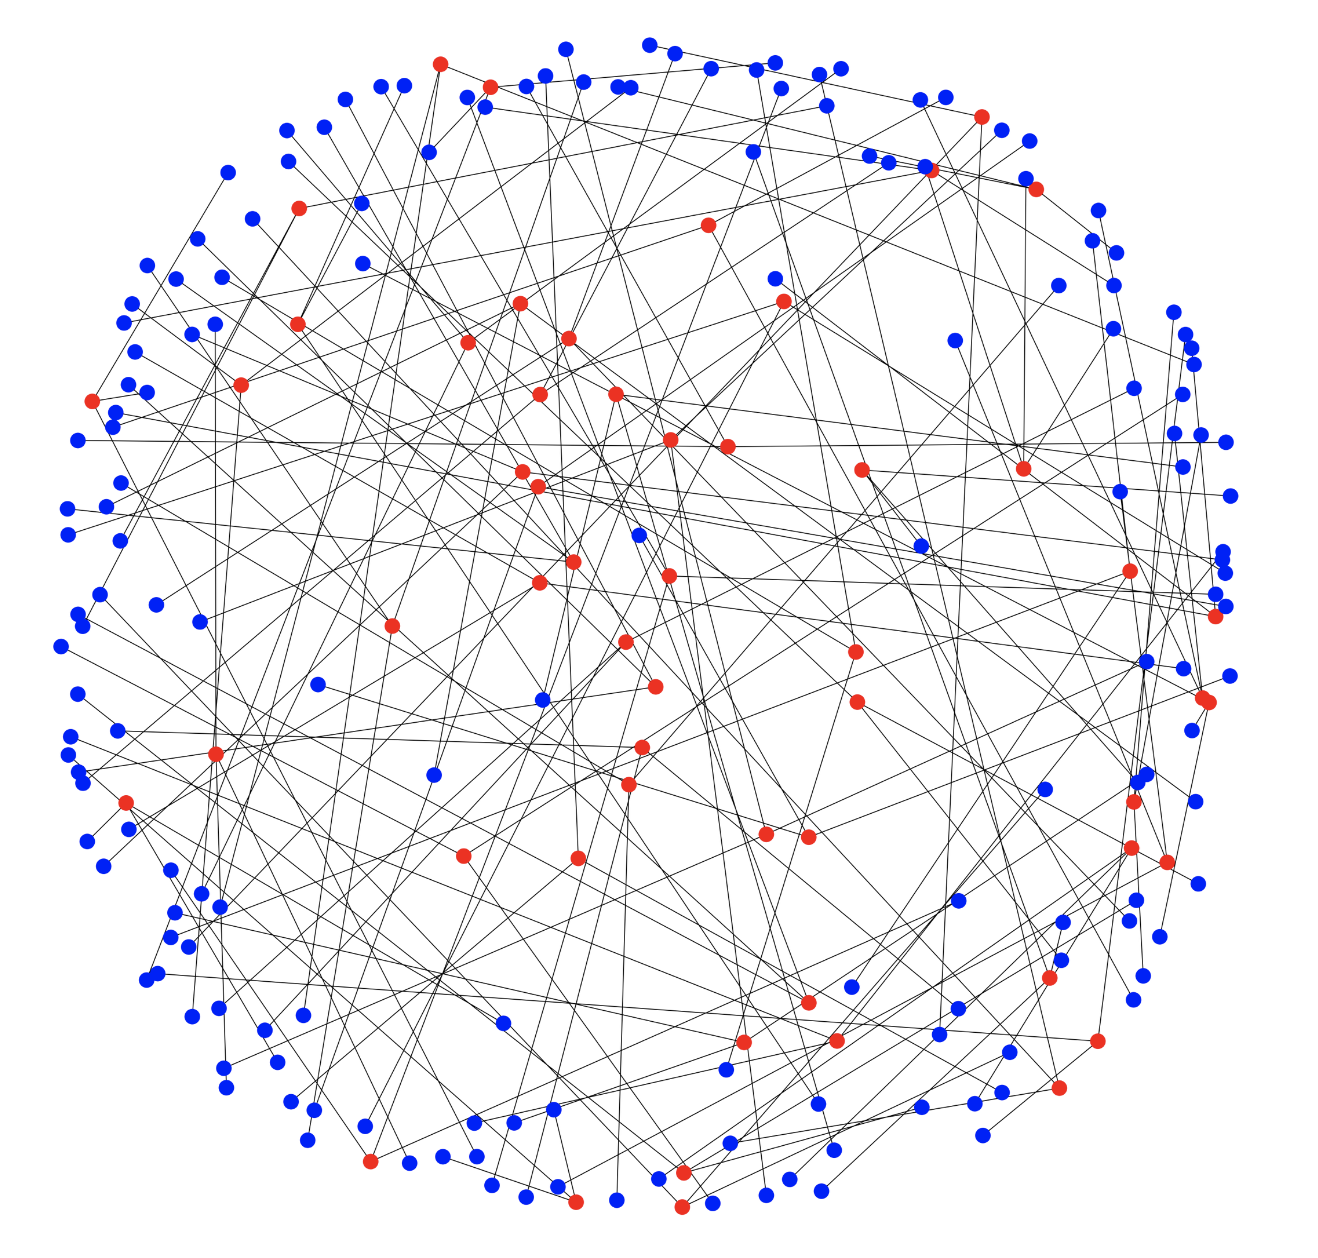
\includegraphics[width=0.49\textwidth]{../paper/img/draw_examples/draw.png}
		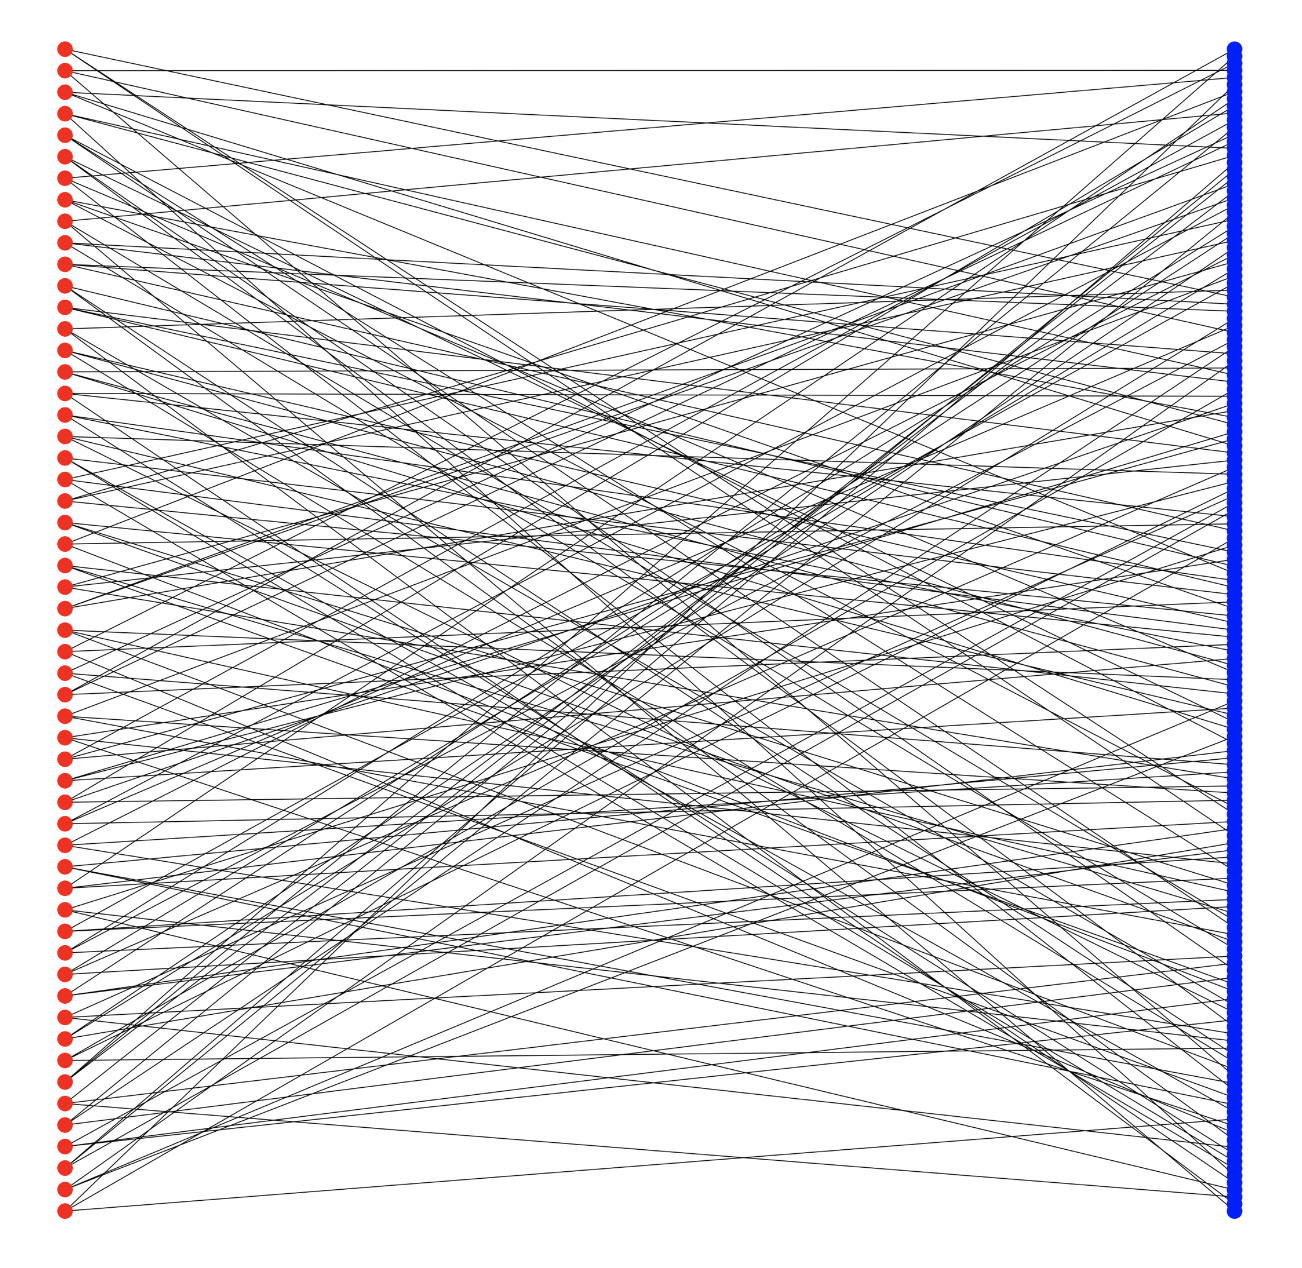
\includegraphics[width=0.49\textwidth]{../paper/img/draw_examples/draw_bipartite.png}
	\end{center}
\end{frame}

\section{Experiments}
\begin{frame}{Experiments}{Overview}
	\begin{itemize}
		\item Hyperparameters $n$, $m$, $p$, $\theta_0$, $\theta_1$, and $\rho$.
	\begin{align}
		\vec{\upmu}_0 \sim \mathcal N(\theta_0, 0.25), \vec{\upmu}_1 \sim \mathcal N(\theta_1, 0.25) \\
		\{\vec{x}_C\}_{j=1}^{m} \sim \mathcal N(\vec{\upmu}_0, \Sigma), \{\vec{x}_T\}_{i=1}^{n} \sim \mathcal N(\vec{\upmu}_1, \Sigma) \\
		\text{ where } \Sigma_{a b} = \begin{cases}
			1 & \text{ if } a = b \\
			\rho & \text{ otherwise.}
		\end{cases}
	\end{align}
		\item Balance metrics: mean ASMD\footnote{Absolute Standardized Mean Difference}, maximum ASMD, proportion of treatment observations matched.
		\begin{itemize}
			\item In practice: use more robust metrics \parencite{basu_use_2008, zhu_kernel-based_2018}.
		\end{itemize}
		\item Vary calipers $c \in \{0.05, 0.10, 0.15, \ldots, 0.50\}$.
	\end{itemize}
\end{frame}


\subsection{Caliper vs. Imbalance}
\begin{frame}{Experiments}{Caliper vs. Imbalance}
	This will consider the effects of increased heterogeneity between $T$ and $C$.
	\begin{itemize}
		\item $m = 750$
		\item $n = 250$
		\item $p = 5$
		\item $\rho = 0$
		\item $\theta_0 = 0$
	\end{itemize}
	We vary $\theta_1 \in \{0, 0.1, 0.2, \ldots, 1\}$.
\end{frame}

\begin{frame}{Experiments}{Caliper vs. Imbalance: Mean Absolute Standardized Mean Difference}
	\begin{center}
		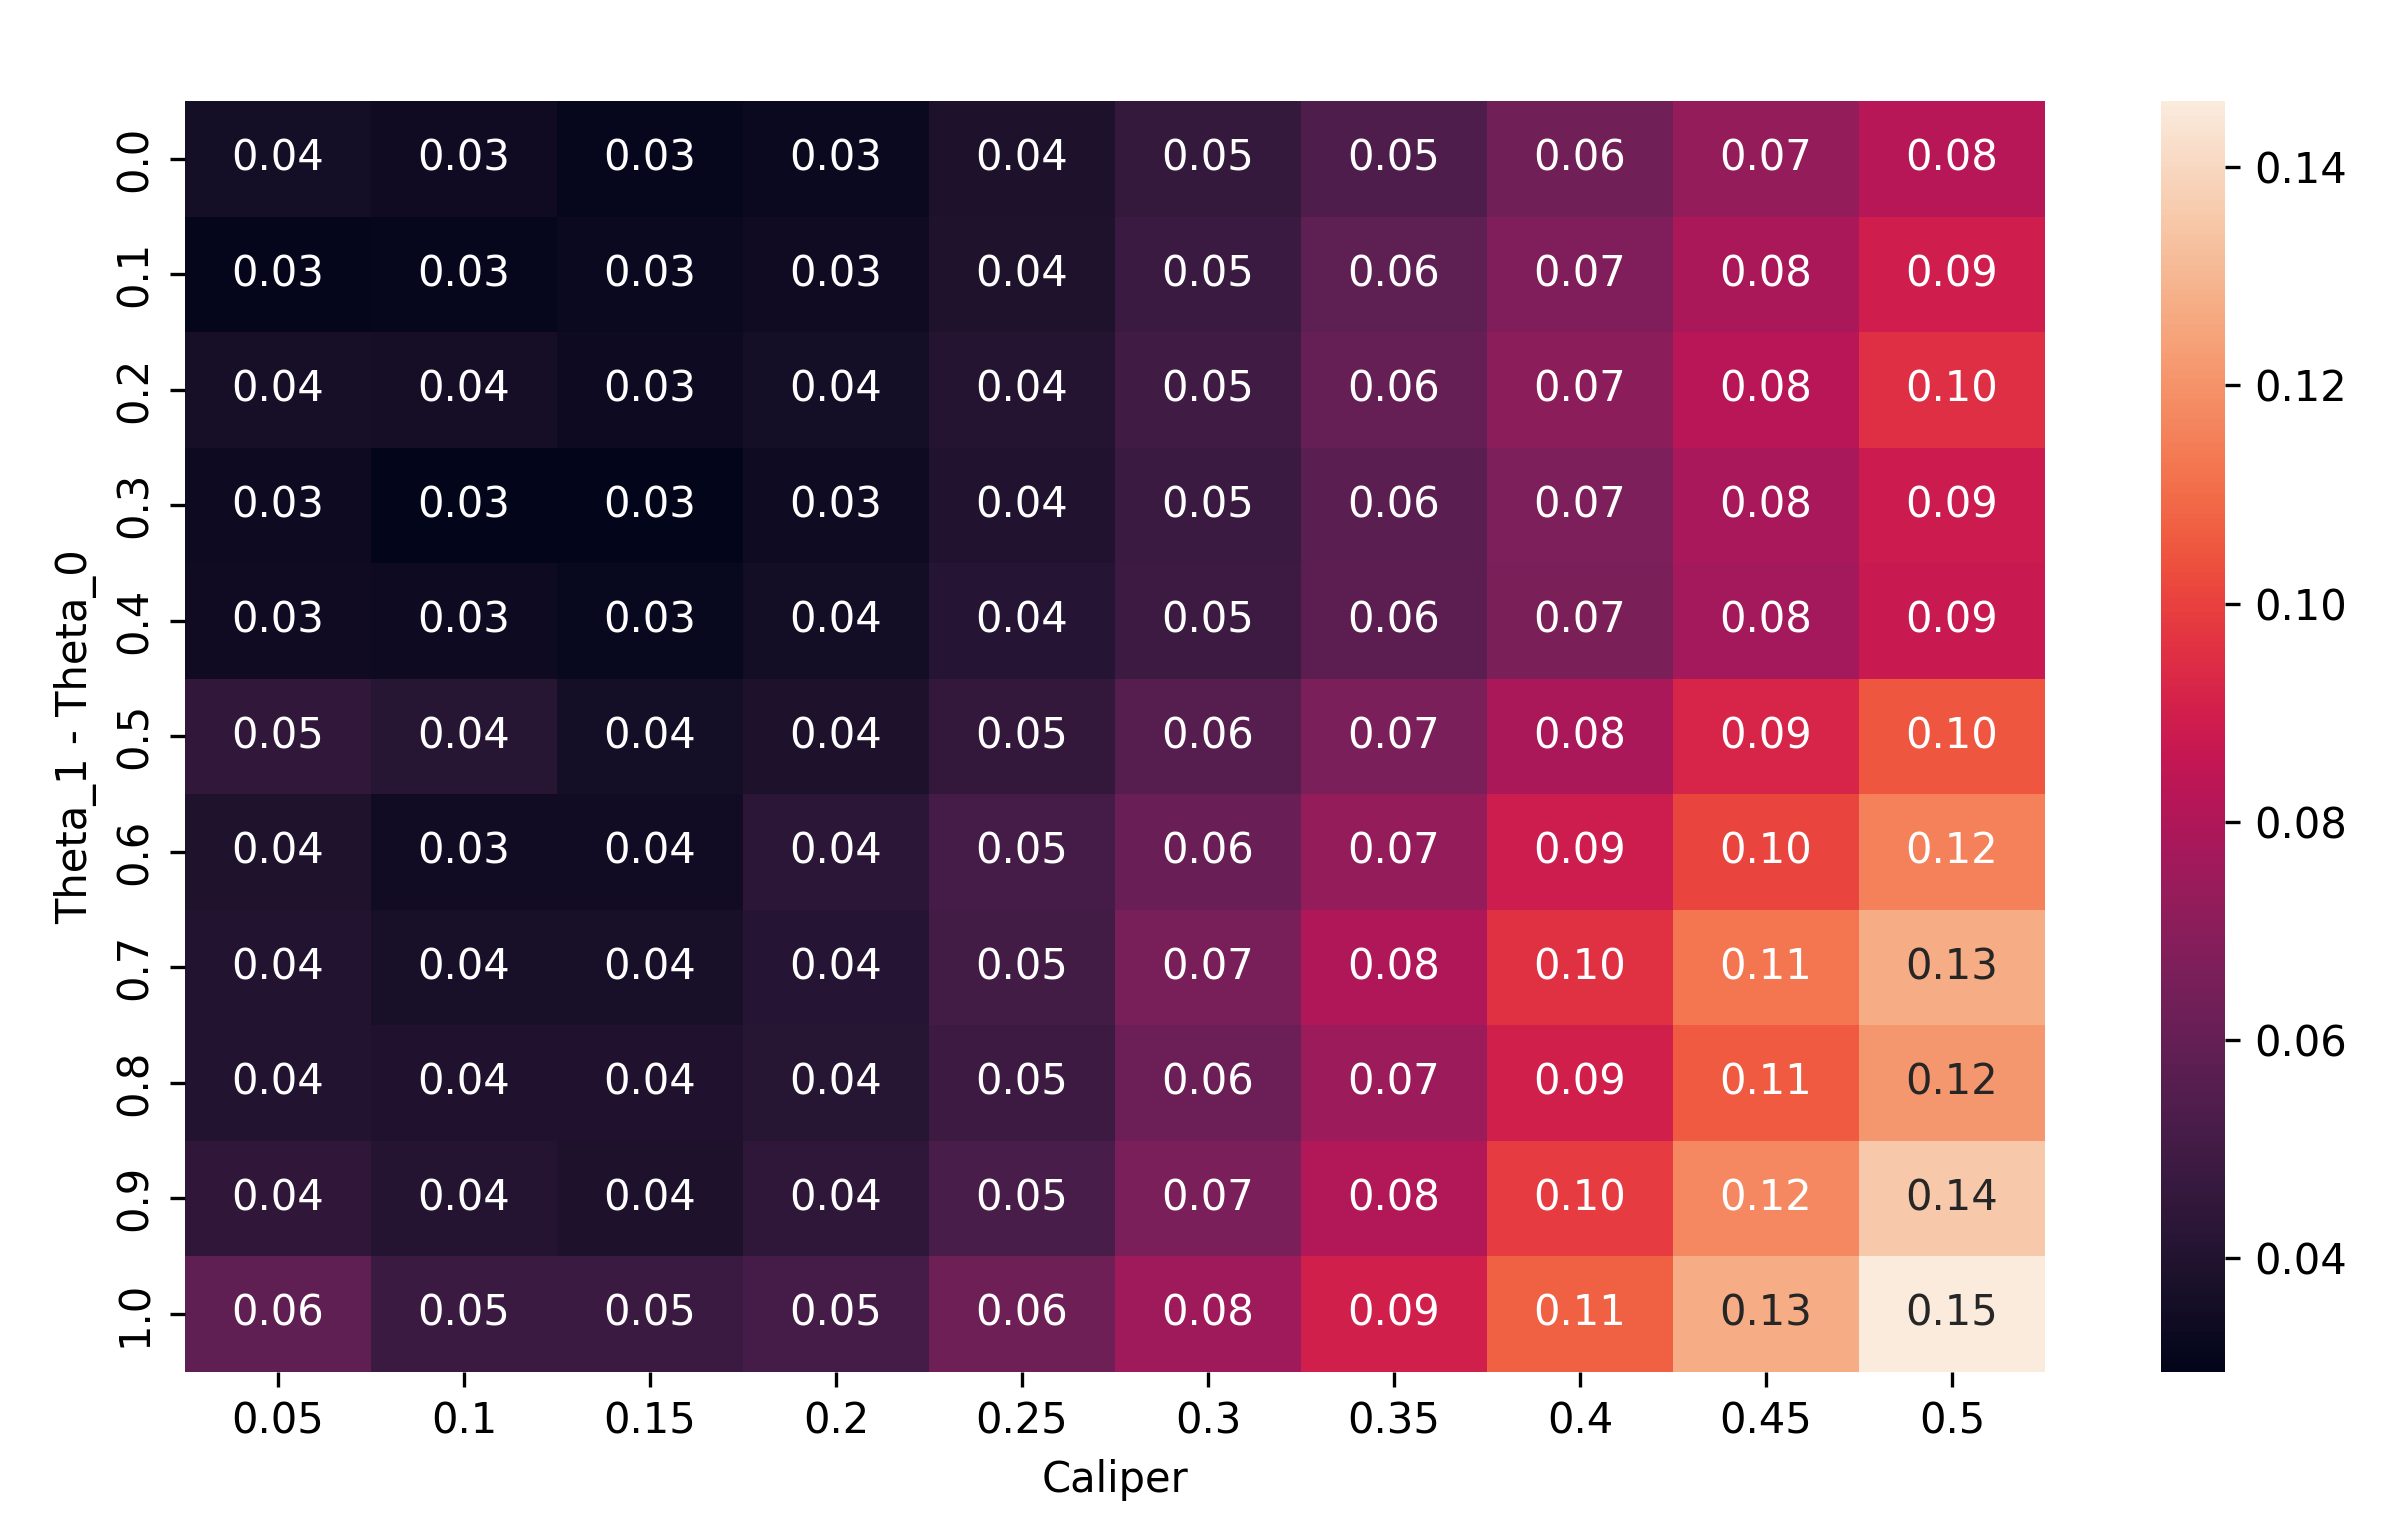
\includegraphics[width=\textwidth]{../paper/img/output30/caliper_vs_imbalance_big/plots/theta1_caliper_mean_abs_smd.png}
	\end{center}
\end{frame}
\begin{frame}{Experiments}{Caliper vs. Imbalance: Maximum Absolute Standardized Mean Difference}
	\begin{center}
		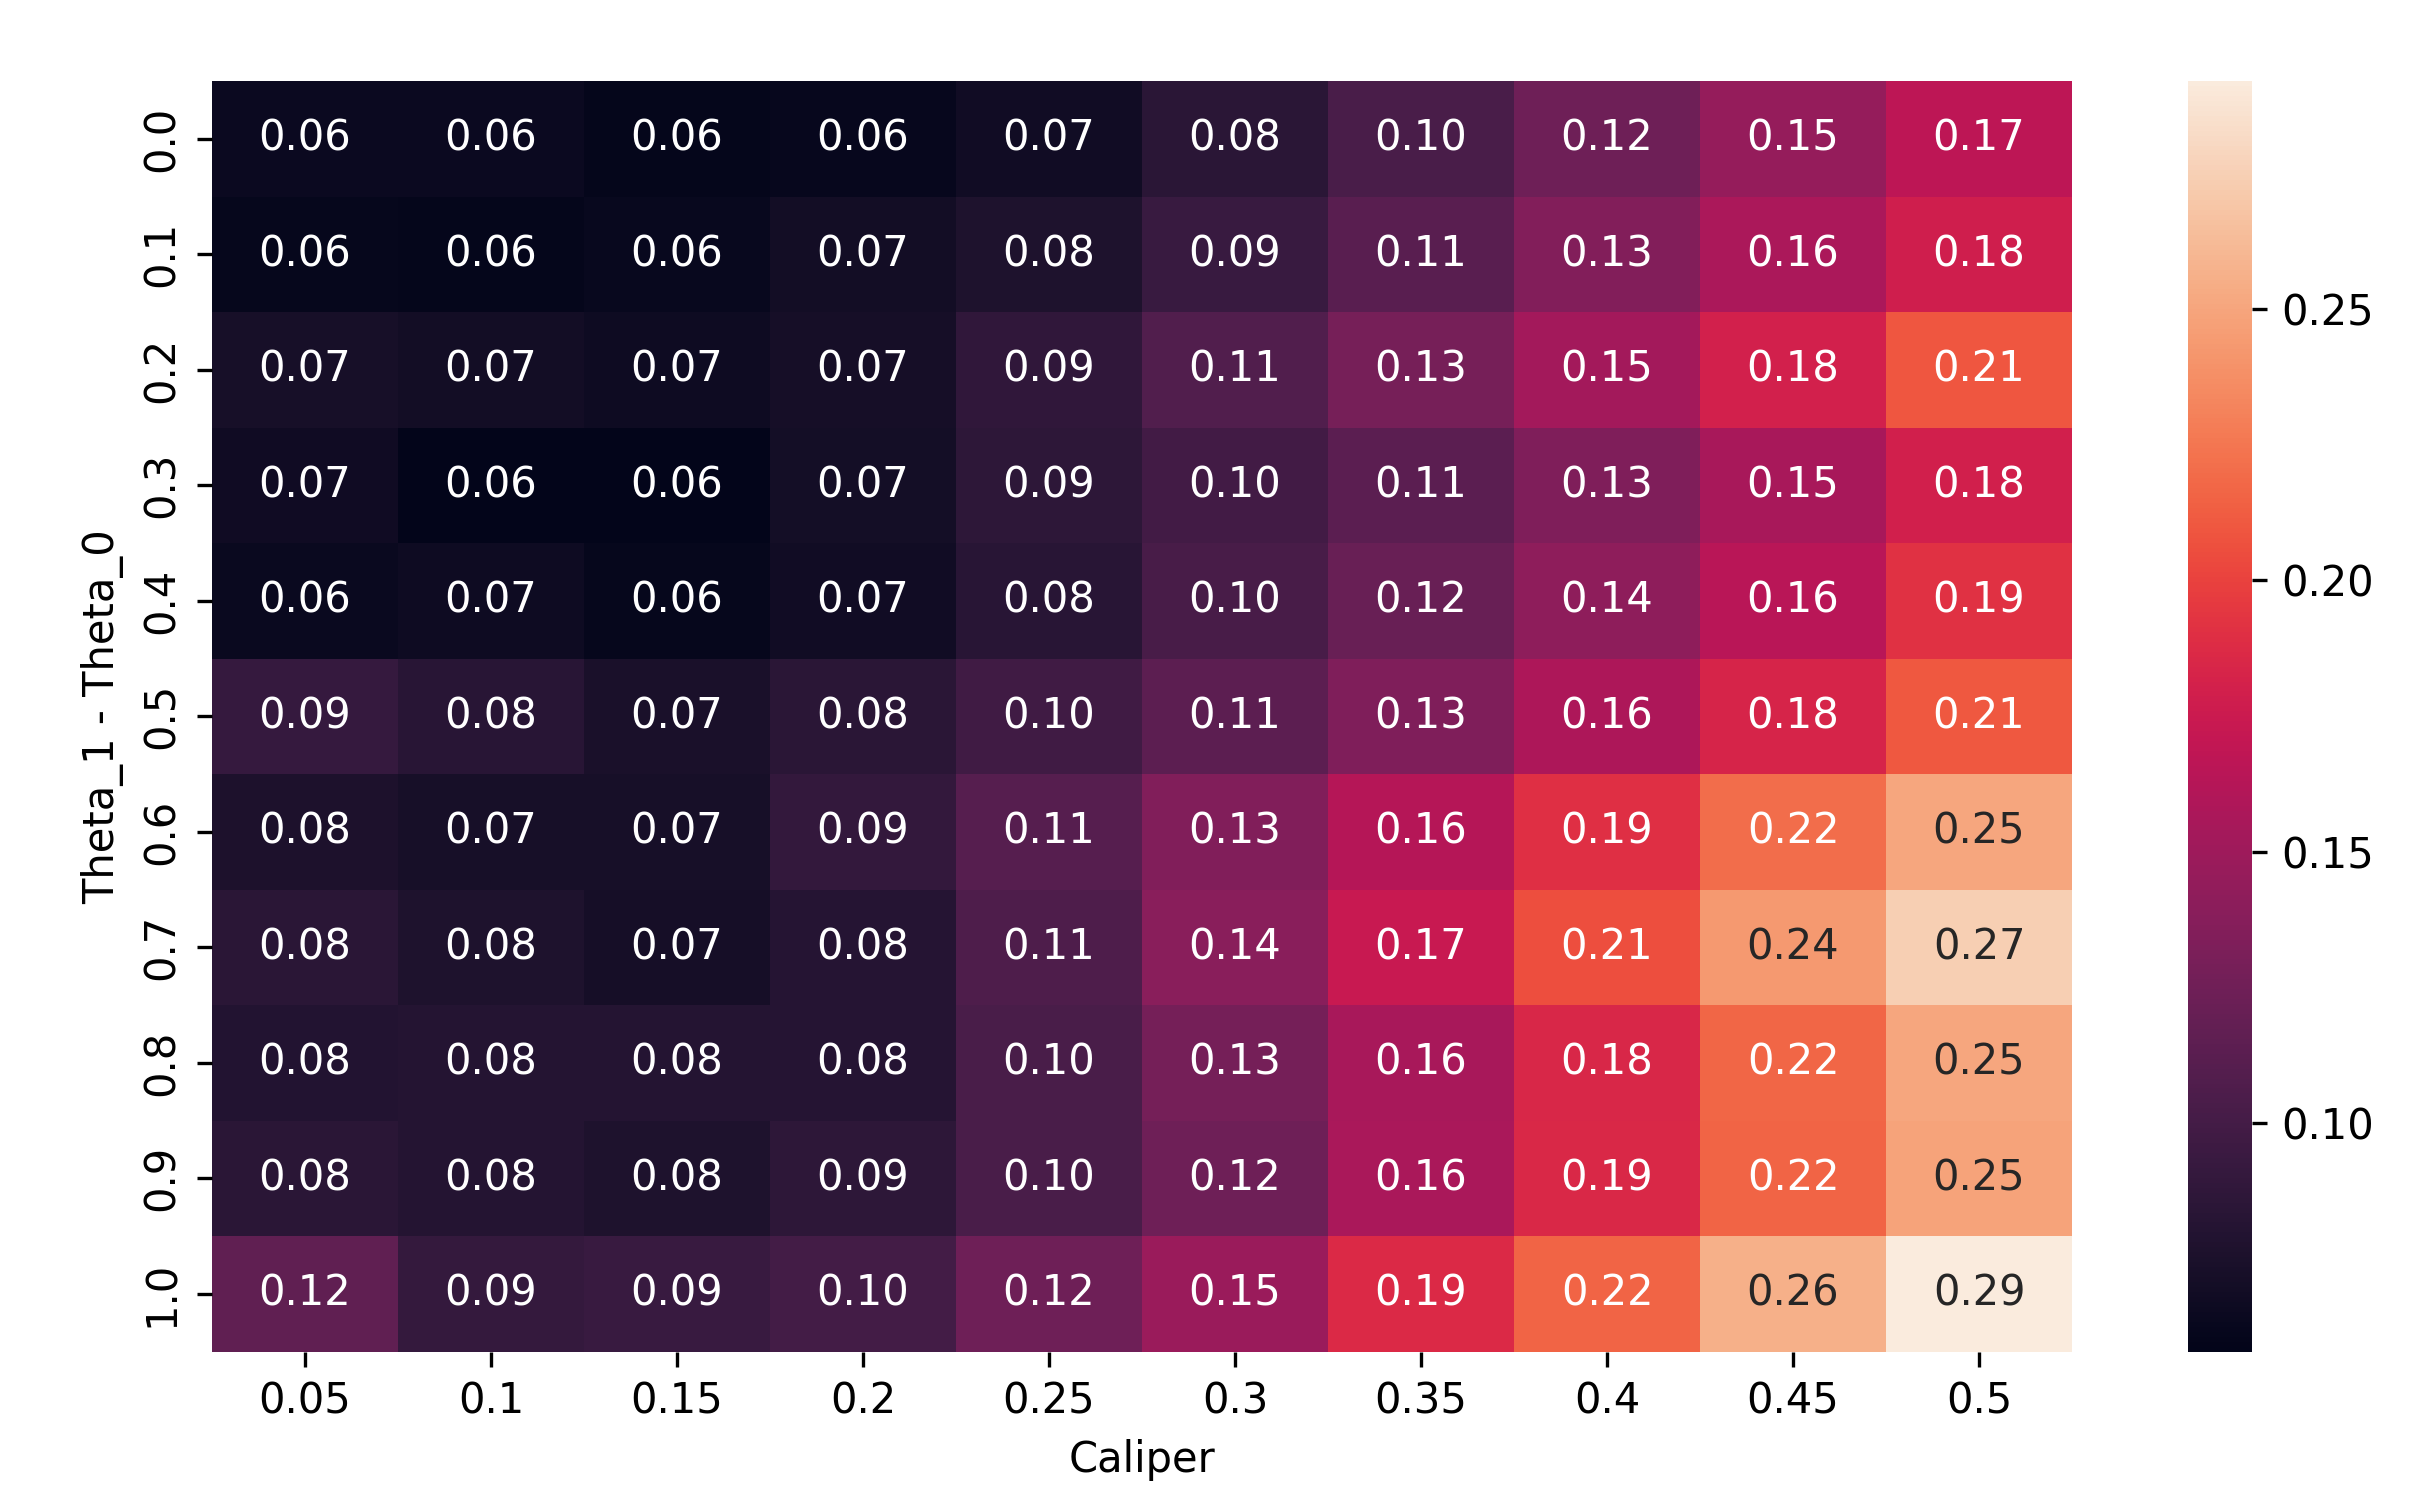
\includegraphics[width=\textwidth]{../paper/img/output30/caliper_vs_imbalance_big/plots/theta1_calipermax_abs_smd.png}
	\end{center}
\end{frame}
\begin{frame}{Experiments}{Caliper vs. Imbalance: Proportion of Treatment Observations Matched}
	\begin{center}
		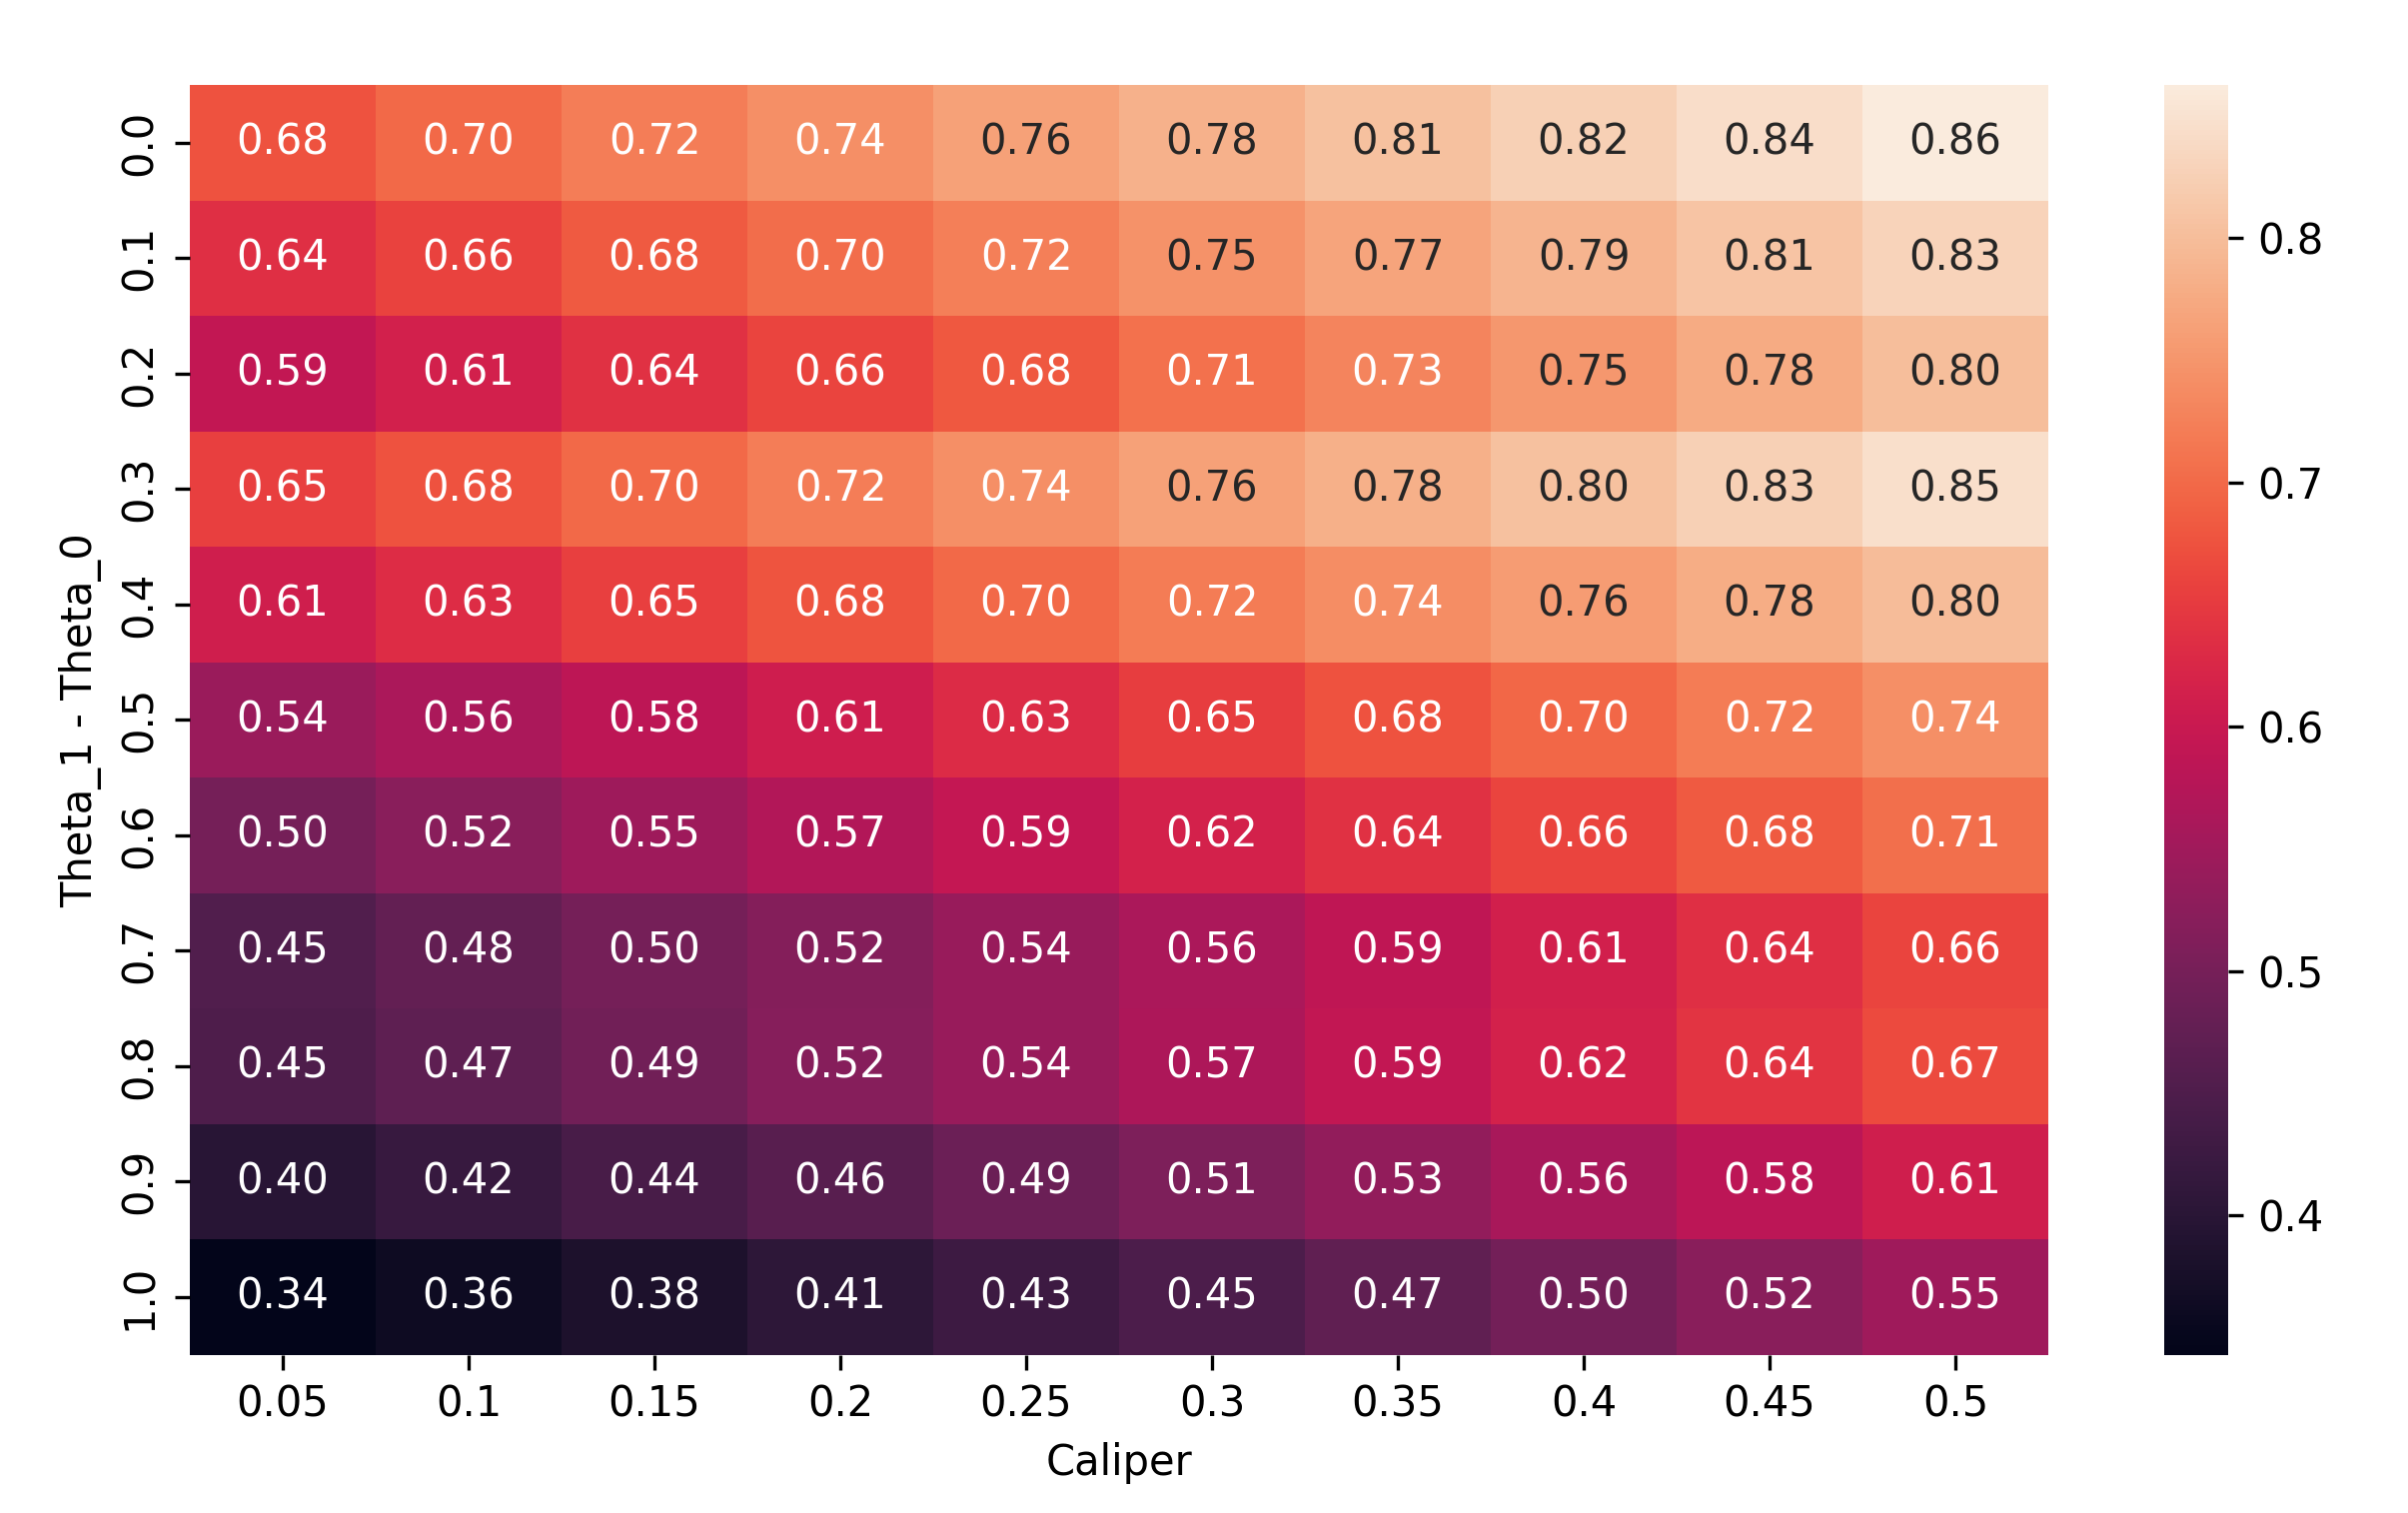
\includegraphics[width=\textwidth]{../paper/img/output30/caliper_vs_imbalance_big/plots/theta1_caliper_prop1_match.png}
	\end{center}
\end{frame}

\subsection{Caliper vs. Correlation}
\begin{frame}{Experiments}{Caliper vs. Correlation}
	This will consider the effects of increased correlation between the features of $X$
	\begin{itemize}
		\item $m = 750$
		\item $n = 250$
		\item $p = 5$
		\item $\theta_0 = 0$
		\item $\theta_1 = 1$
	\end{itemize}
	We vary $\rho \in \{0, 0.1, 0.2, \ldots, 0.8\}$.
\end{frame}
\begin{frame}{Experiments}{Caliper vs. Correlation: Mean Absolute Standardized Mean Difference}
	\begin{center}
		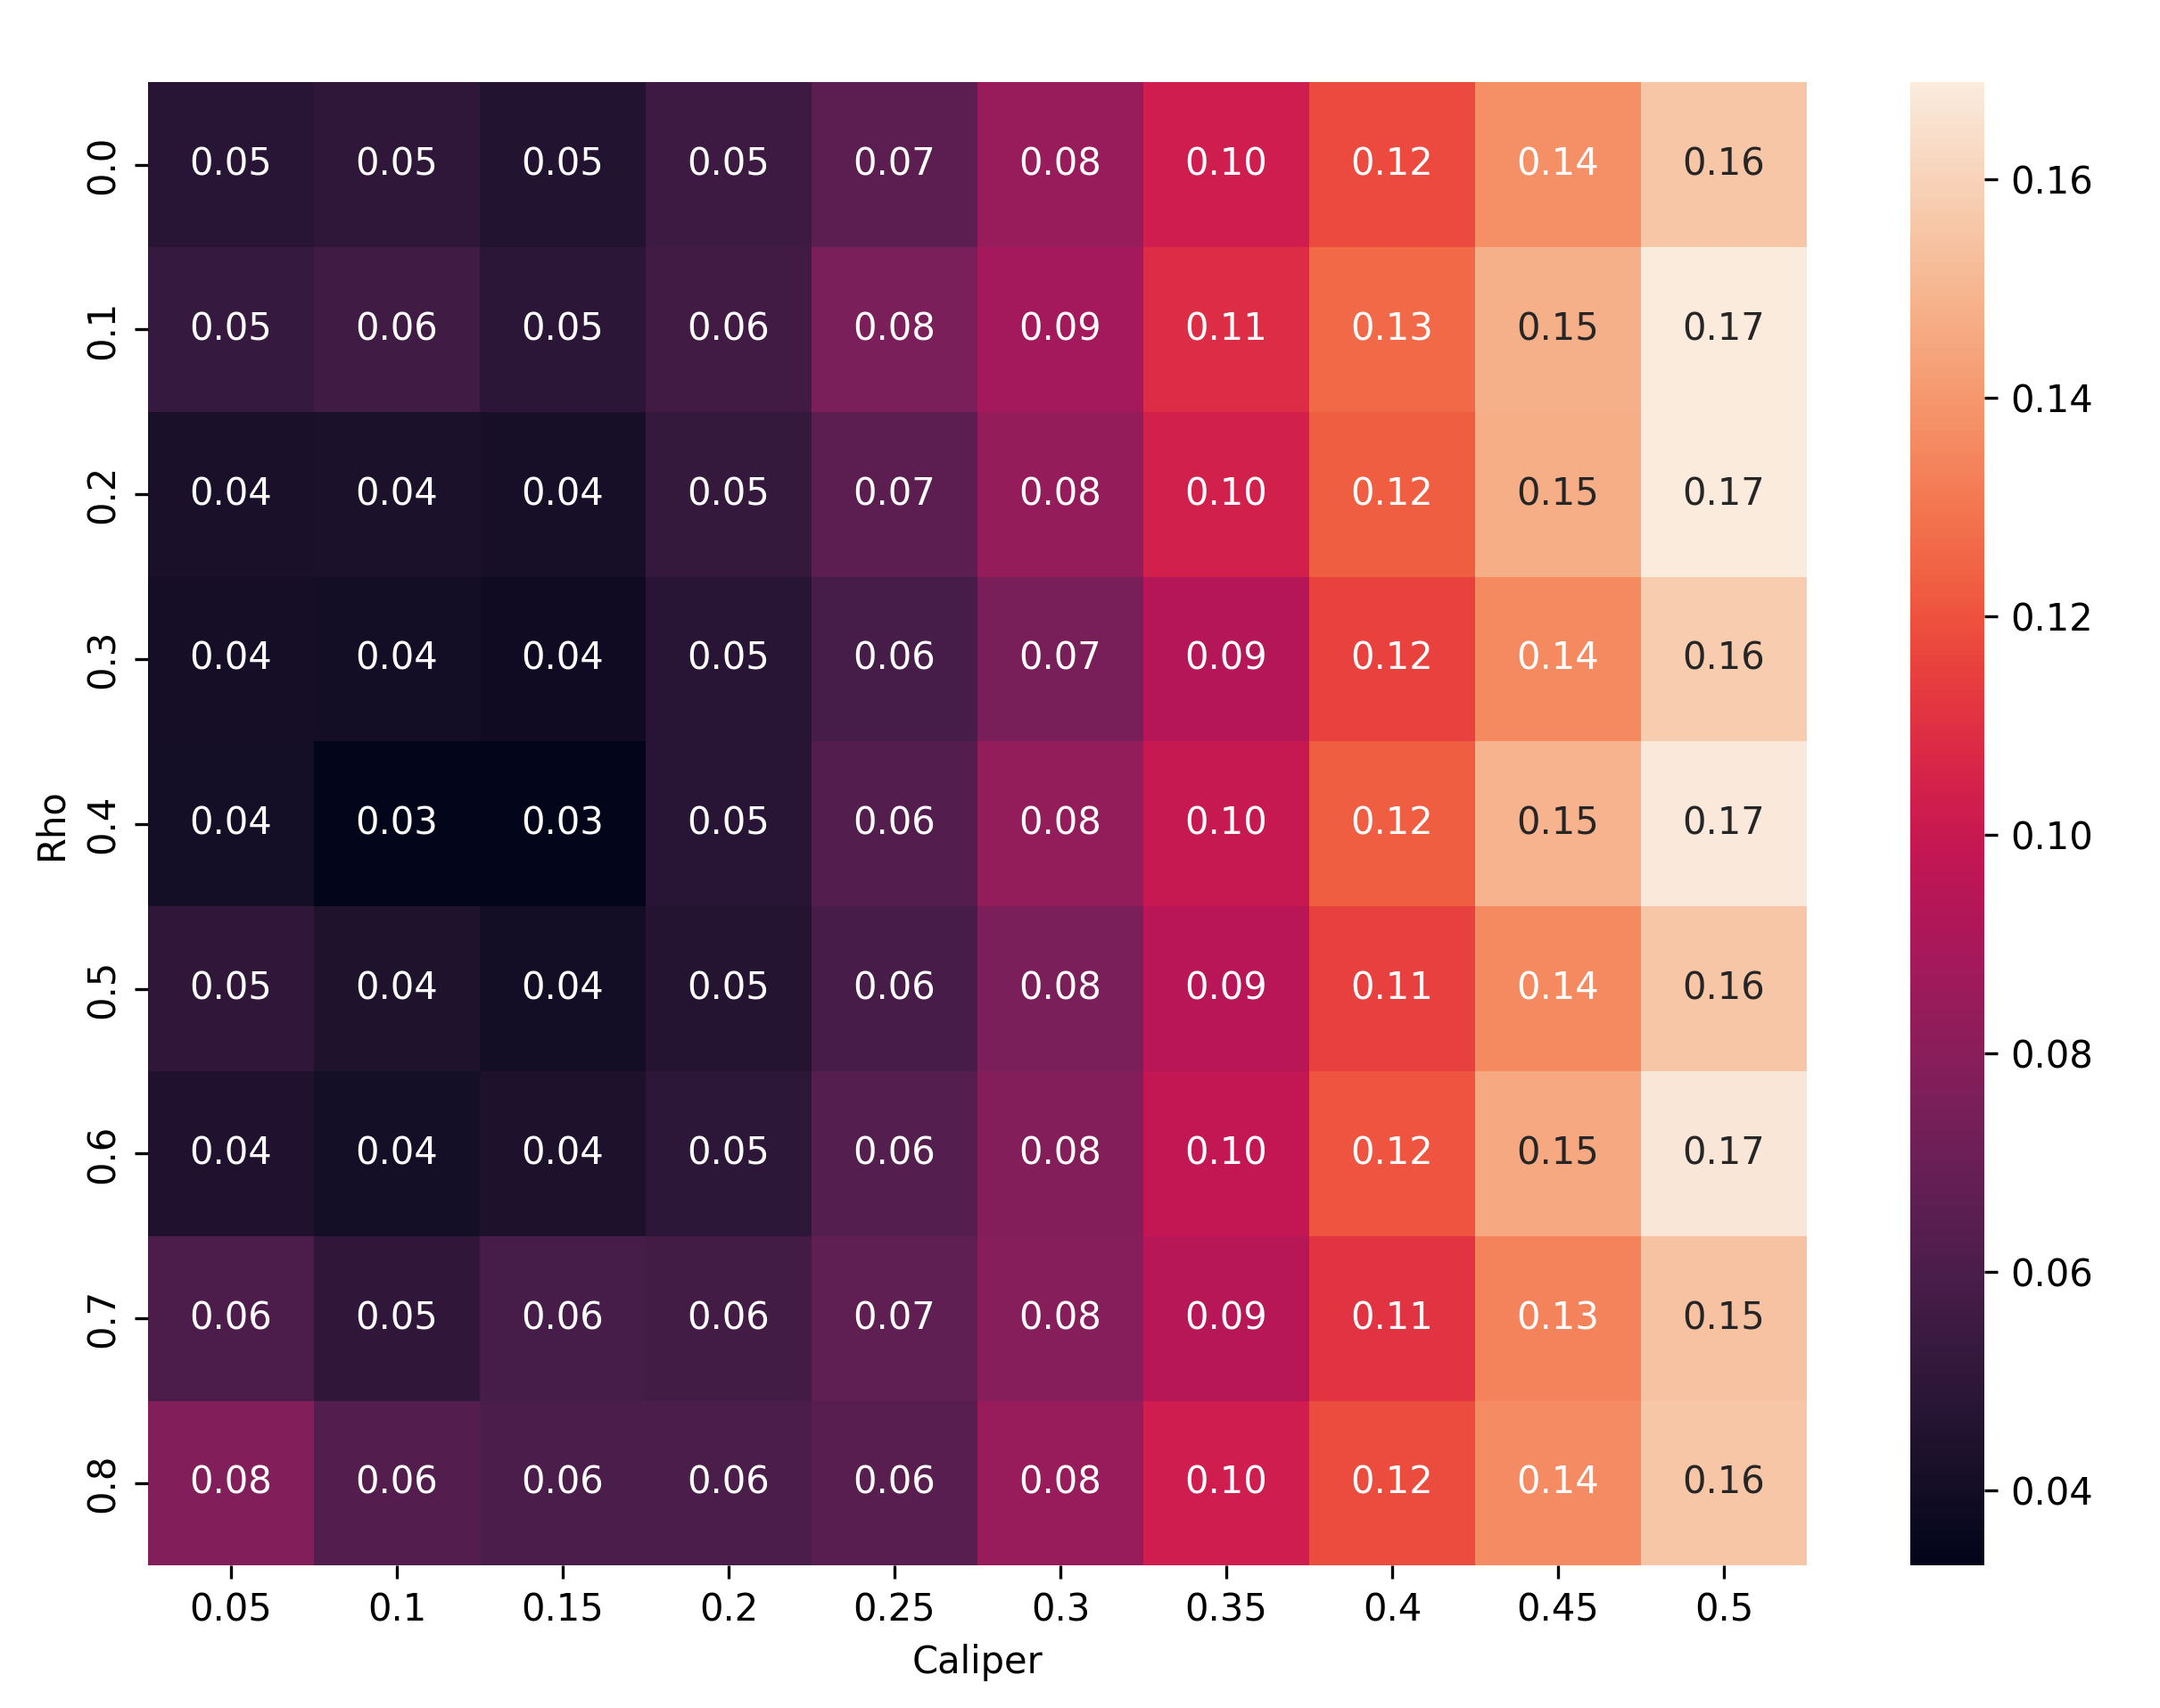
\includegraphics[width=\textwidth]{../paper/img/output30/caliper_vs_correlation_big/plots/rho_caliper_mean_abs_smd.png}
	\end{center}
\end{frame}
\begin{frame}{Experiments}{Caliper vs. Correlation: Maximum Absolute Standardized Mean Difference}
	\begin{center}
		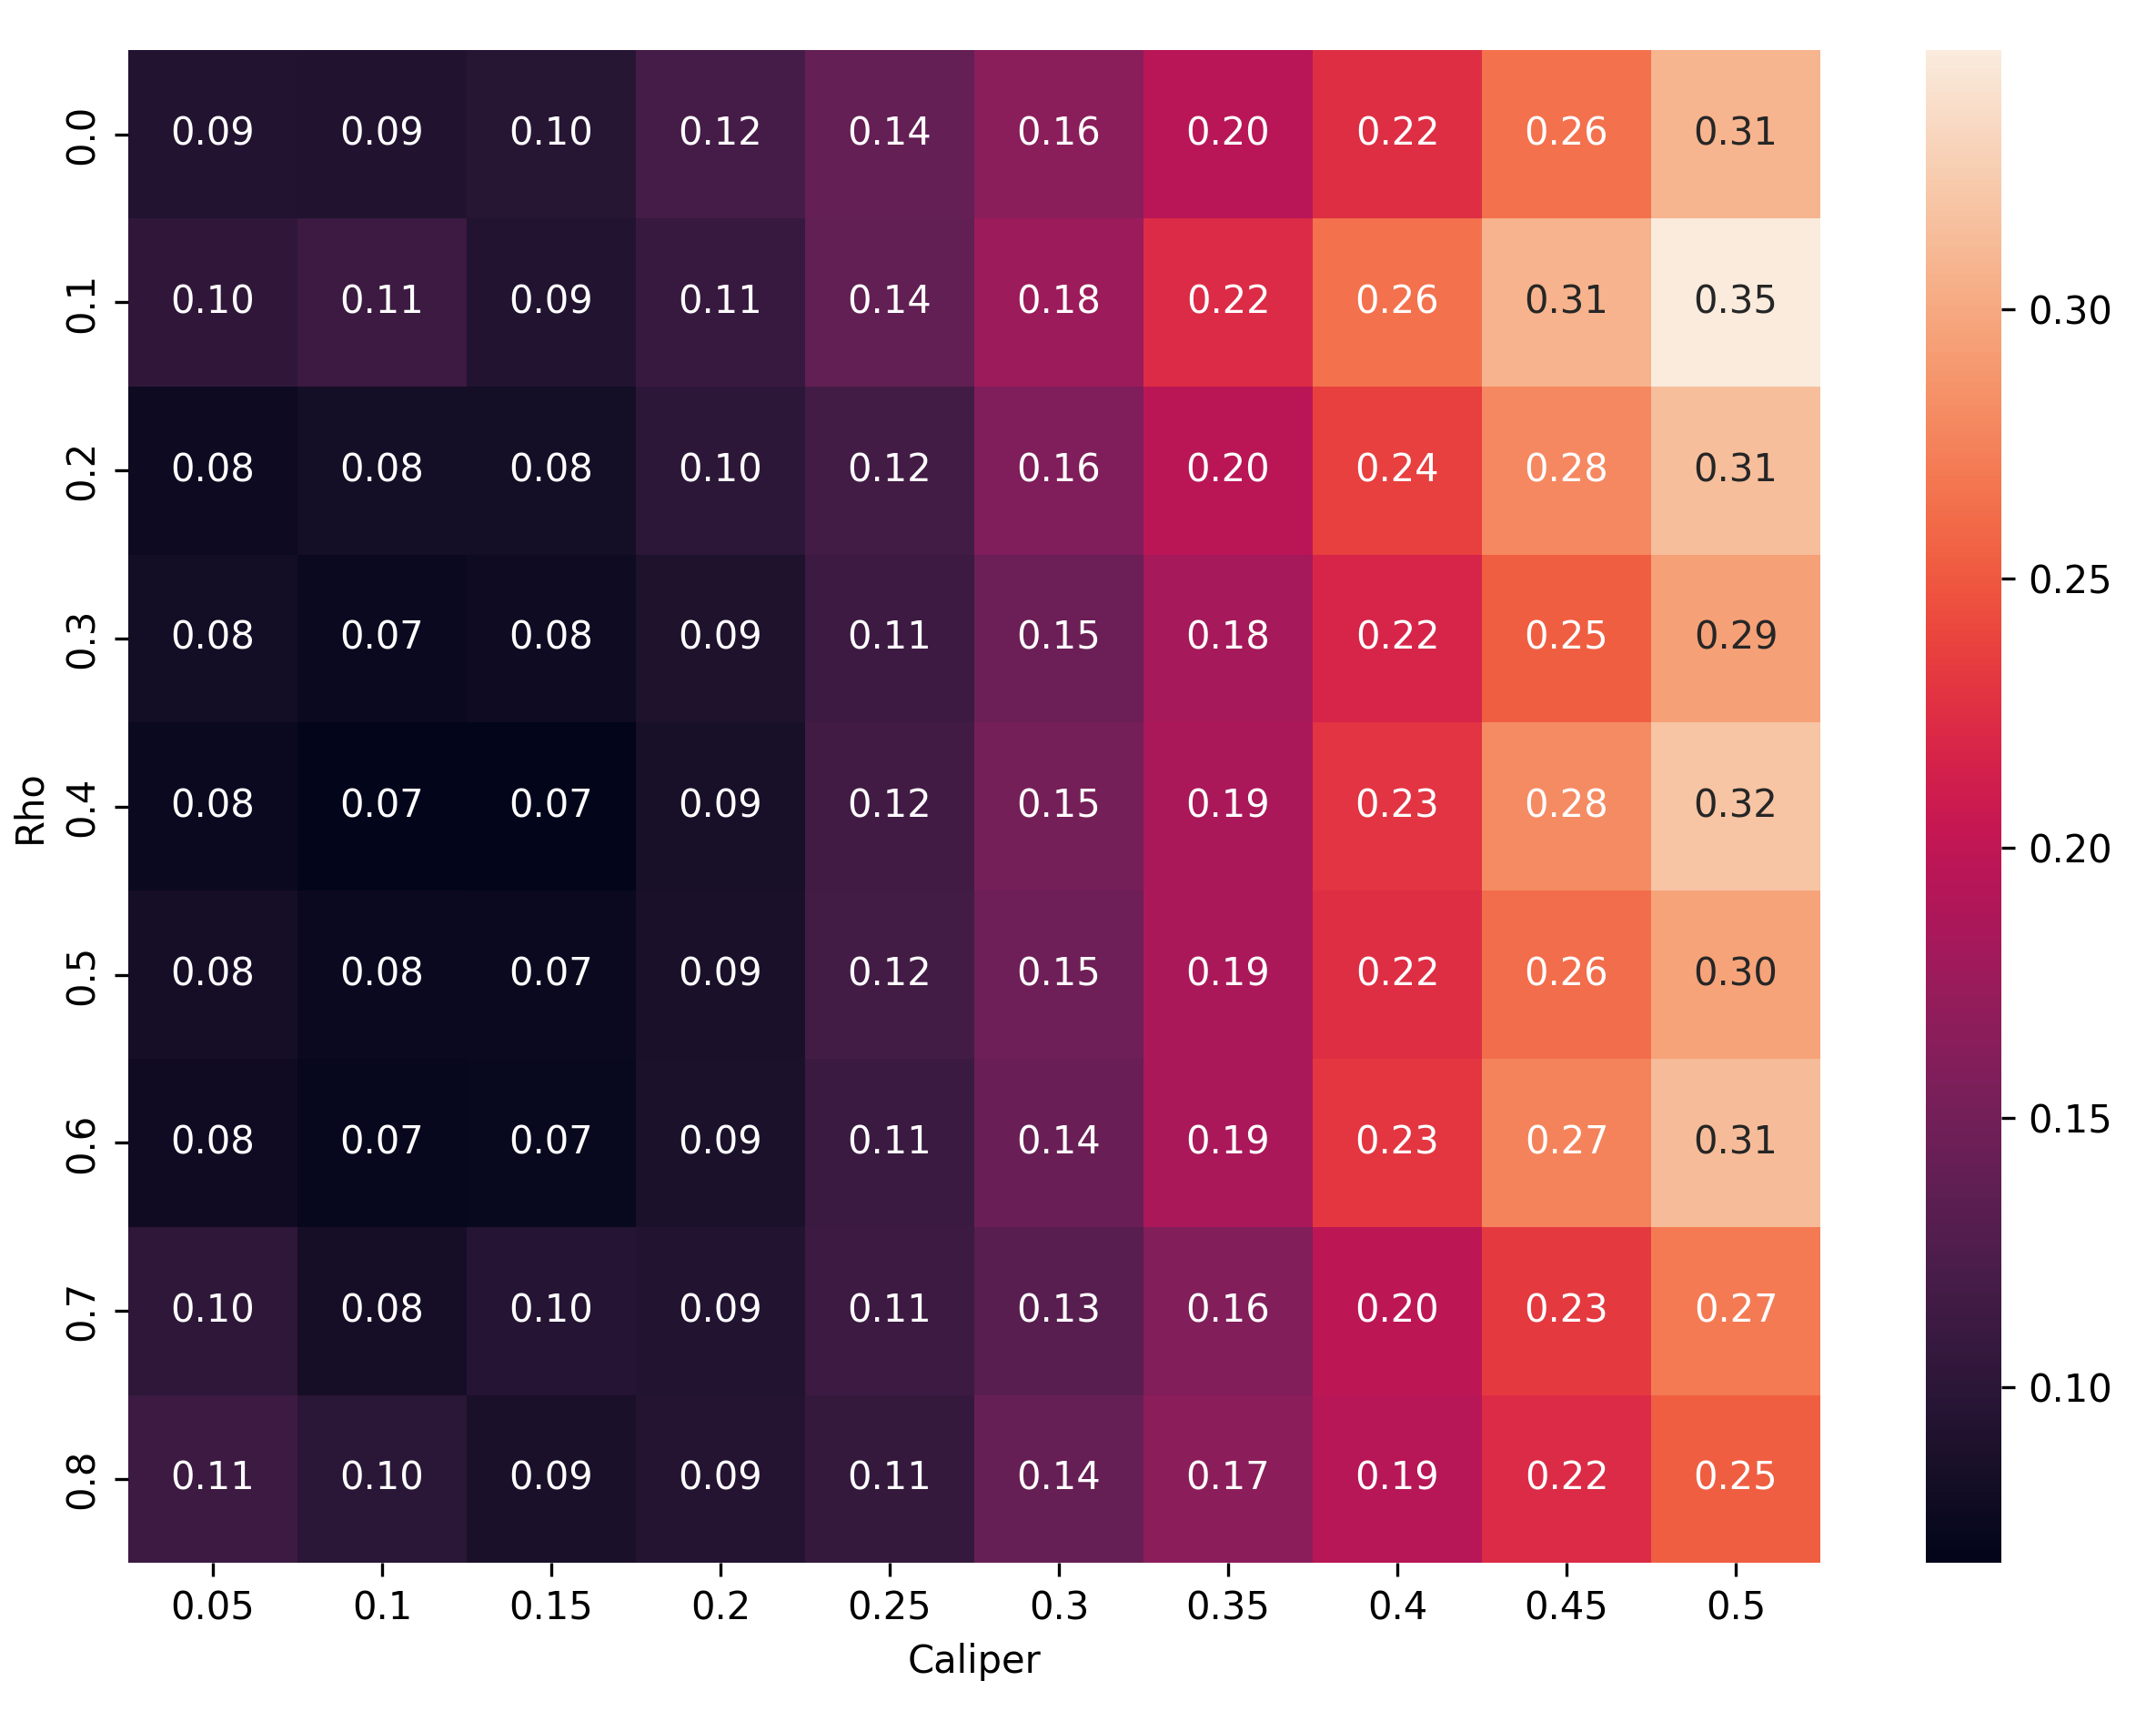
\includegraphics[width=\textwidth]{../paper/img/output30/caliper_vs_correlation_big/plots/rho_calipermax_abs_smd.png}
	\end{center}
\end{frame}
\begin{frame}{Experiments}{Caliper vs. Correlation: Proportion of Treatment Observations Matched}
	\begin{center}
		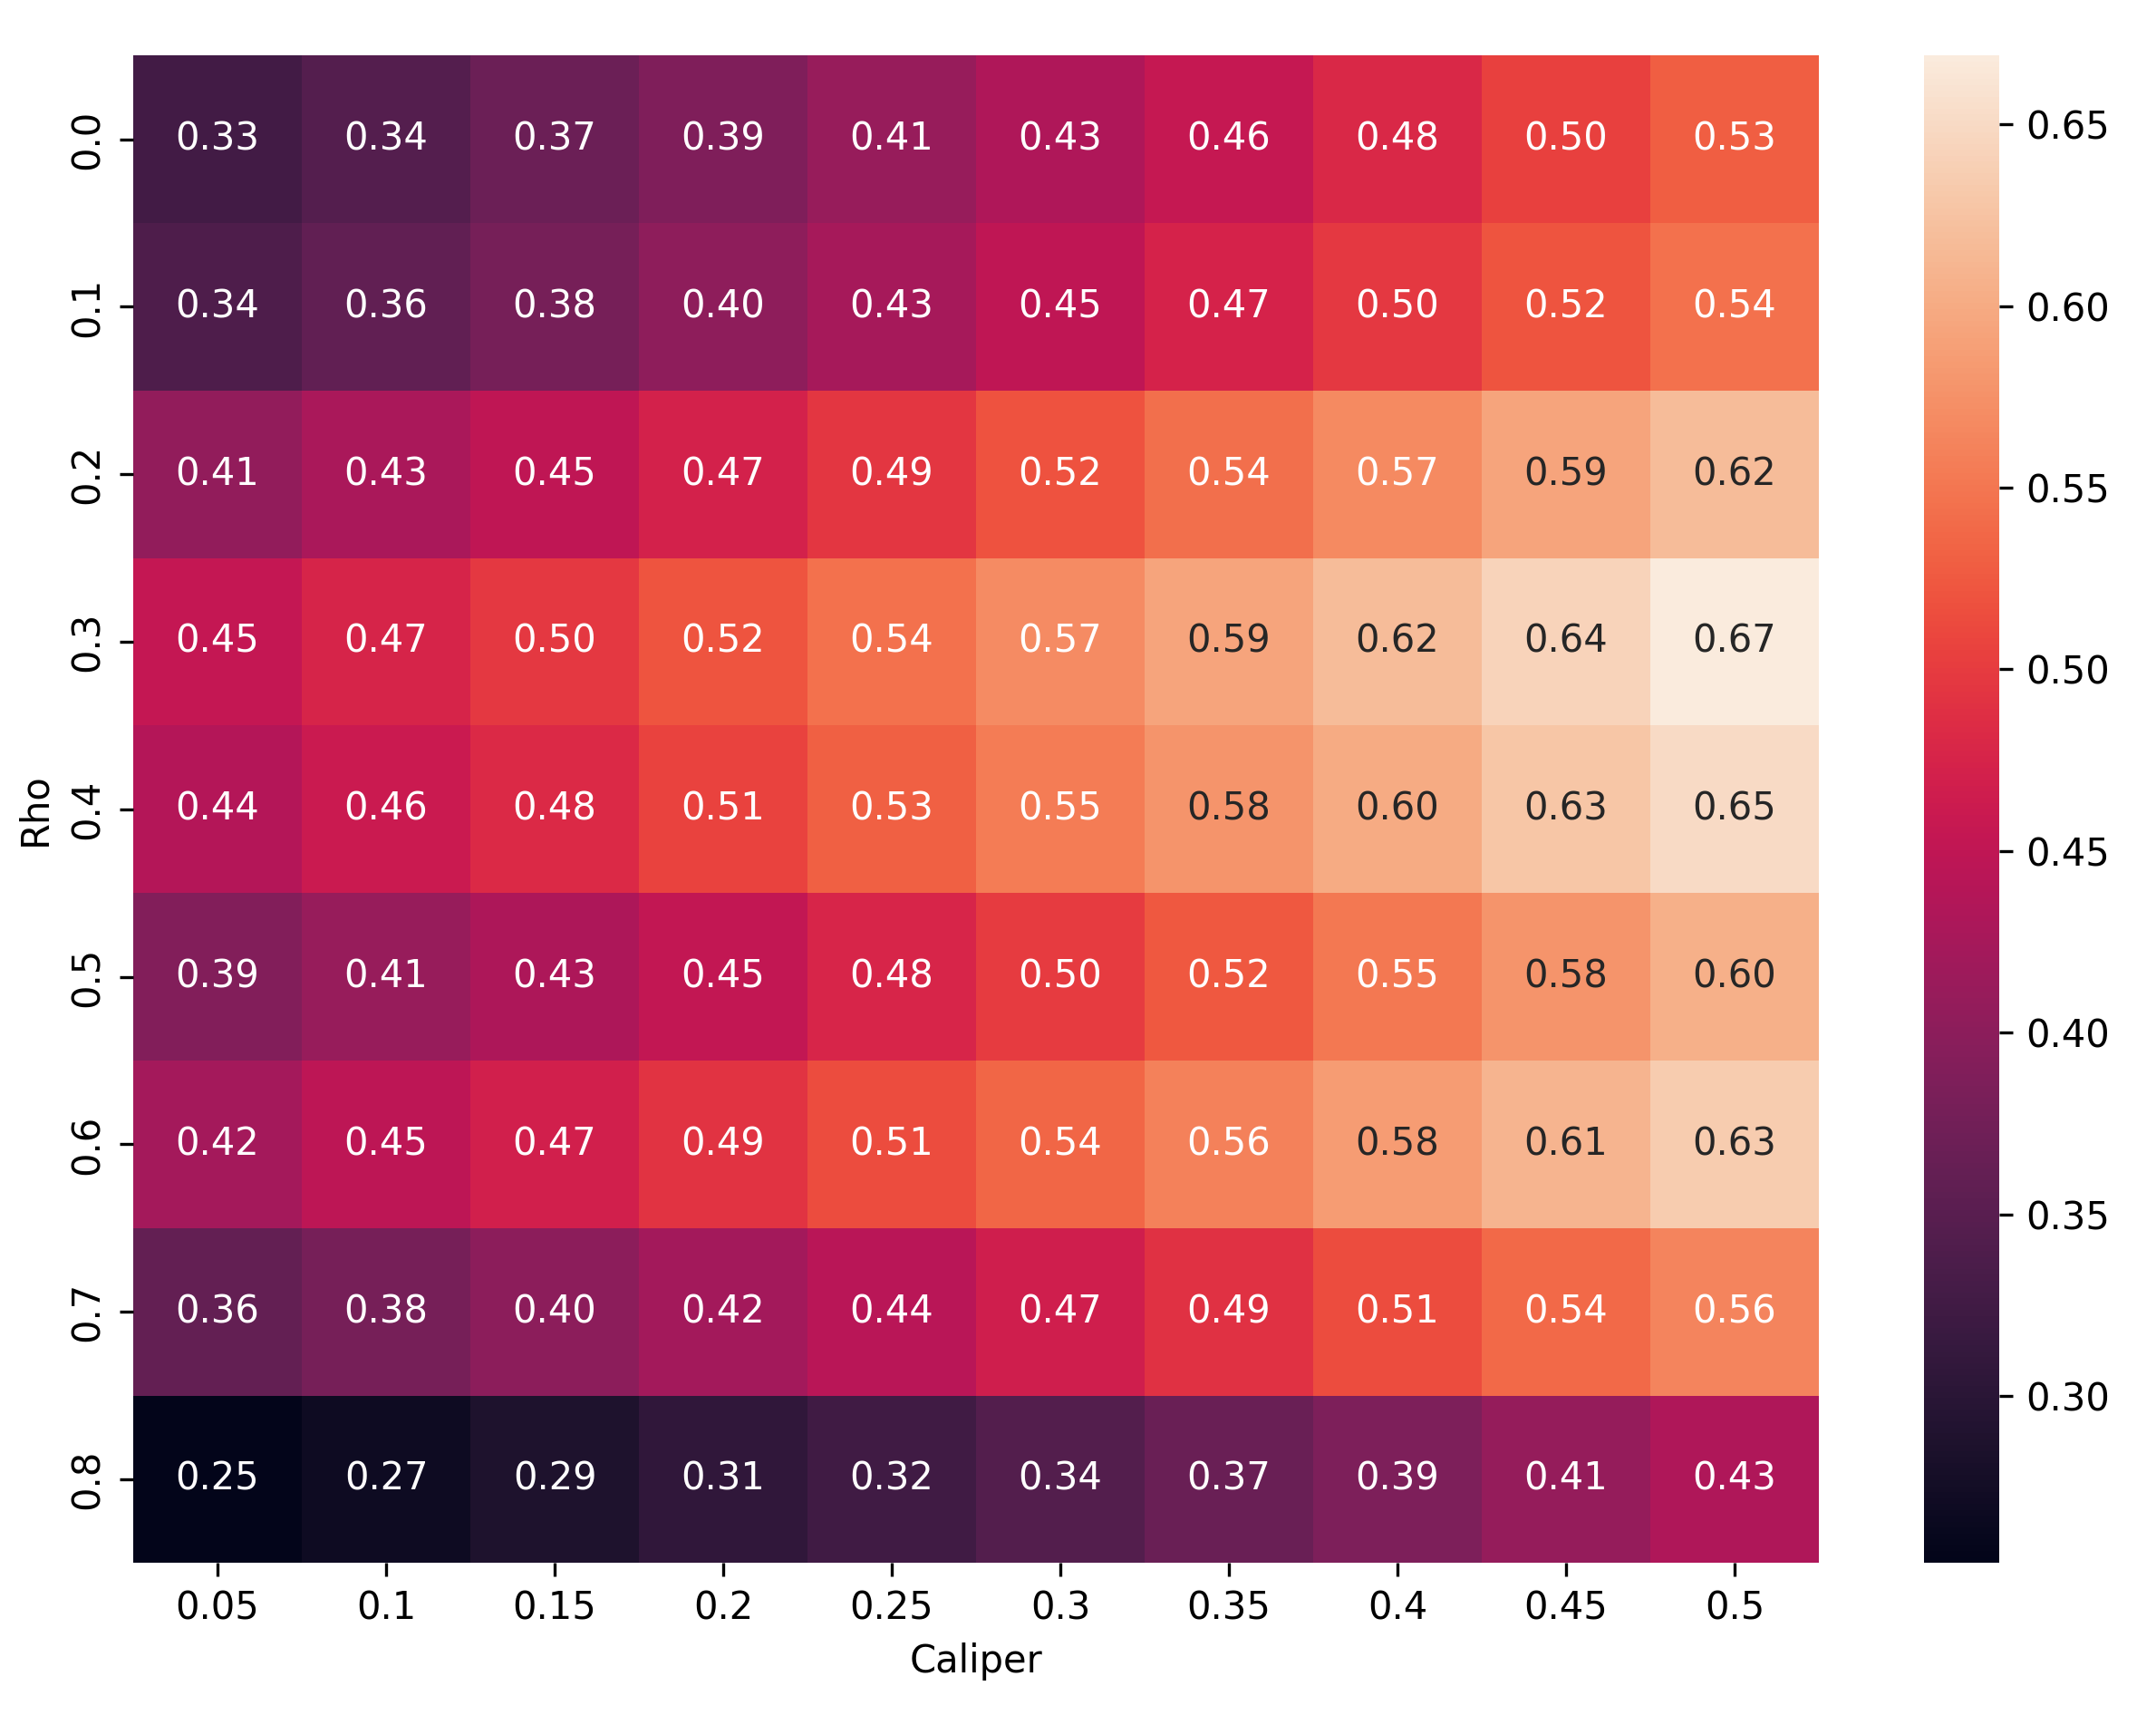
\includegraphics[width=\textwidth]{../paper/img/output30/caliper_vs_correlation_big/plots/rho_caliper_prop1_match.png}
	\end{center}
\end{frame}

\section{Conclusion}
\begin{frame}{Conclusion}
	\begin{itemize}
		\item Common theme of numerical studies: data-dependence.
		\item Emphasizes the importance of
			\begin{itemize}
				\item quality of balance metrics;
				\item inspectability of matching.
			\end{itemize}
		\item \texttt{matching} offers extreme flexibility in design of matching process.
			\begin{itemize}
				\item The current state of the graph is always inspectable.
				\item Can easily tune matches.
			\end{itemize}
	\end{itemize}
\end{frame}


\begin{frame}[fragile]
\frametitle{\texttt{matching} Example Code}
\begin{minted}[escapeinside=||, linenos, fontsize=\scriptsize]{python3}
from matplotlib import pyplot as plt
from matching.distance import Exact, L1Norm
from matching.graph import MatchingGraph
from matching.preprocessing import propensity_score

# Take `caliper_width` as given
# `X` has columns "score" and "is_nice", `z` is treatment assignments
mg = MatchingGraph(X, z)

# NOTE: there is also a keyword argument "exclude"
mg.set_edges(distance=L1Norm(max_distance=caliper_width), include=["score"])
mg.filter_edges(distance=Exact(), include=["is_nice"])

# Conduct optimal matching
mg.match(n_match=3, min_match=3, method="optimal")

# Get the matched data as a `pandas.DataFrame`
match_df = mg.match_data.frame

# Draw the graph of matches
mg.draw()
plt.show()
\end{minted}
\end{frame}

% \section*{References}
% \begin{frame}[allowframebreaks]
% 	\frametitle{References}
% 	\printbibliography
% \end{frame}


\end{document}
